\documentclass[final]{fhnwreport}       %[mode] = draft or final
                                        %{class} = fhnwreport, article, 
                                        %          report, book, beamer, standalone
%%---Main Packages-----------------------------------------------------------------------
\usepackage[english, ngerman]{babel}	%Mul­tilin­gual sup­port for LaTeX
\usepackage[T1]{fontenc}				%Stan­dard pack­age for se­lect­ing font en­cod­ings
\usepackage[utf8]{inputenc}				%Ac­cept dif­fer­ent in­put en­cod­ings
\usepackage{lmodern}                    %The newer Font-Set
\usepackage{textcomp}					%LaTeX sup­port for the Text Com­pan­ion fonts
\usepackage{graphicx} 					%En­hanced sup­port for graph­ics
\usepackage{float}						%Im­proved in­ter­face for float­ing ob­jects
\usepackage{ifdraft}                    %Let you check if the doc is in draft mode

%%---Useful Packages---------------------------------------------------------------------
\usepackage[pdftex,dvipsnames,table]{xcolor}  %Driver-in­de­pen­dent color ex­ten­sions for LaTeX
\usepackage{csquotes}                   %Simpler quoting with \enquote{}
\usepackage{siunitx} 					%A com­pre­hen­sive (SI) units pack­age
\usepackage{listings}					%Type­set source code list­ings us­ing LaTeX
\usepackage[bottom]{footmisc}			%A range of foot­note op­tions
\usepackage{footnote}					%Im­prove on LaTeX's foot­note han­dling
\usepackage{verbatim}					%Reim­ple­men­ta­tion of and ex­ten­sions to LaTeX ver­ba­tim
\usepackage[textsize=footnotesize]{todonotes} %Mark­ing things to do in a LaTeX doc­u­ment
\usepackage{booktabs}
\usepackage{lscape}
\usepackage{blindtext}
\usepackage{wrapfig}
\usepackage{caption}
\usepackage{romannum}

%%---Tikz Packages-----------------------------------------------------------------------
\usepackage{standalone}
\usepackage{tikz}
\usepackage{circuitikz}
\usetikzlibrary{arrows}
\usetikzlibrary{calc}
\usetikzlibrary{intersections}

%%---Math Packages-----------------------------------------------------------------------
\usepackage{amsmath}					%AMS math­e­mat­i­cal fa­cil­i­ties for LaTeX
%\usepackage{amssymb}					%Type­set­ting symbols (AMS style)
%\usepackage{array}						%Ex­tend­ing the ar­ray and tab­u­lar en­vi­ron­ments
%\usepackage{amsthm}					%Type­set­ting the­o­rems (AMS style)

%%---Table Packages----------------------------------------------------------------------
\usepackage{tabularx}					%Tab­u­lars with ad­justable-width columns
%\usepackage{longtable}
\usepackage{multirow}					%Create tab­u­lar cells span­ning mul­ti­ple rows
\usepackage{multicol}					%In­ter­mix sin­gle and mul­ti­ple columns

%%---PDF / Figure Packages---------------------------------------------------------------
\usepackage{pdfpages}					%In­clude PDF doc­u­ments in LaTeX
\usepackage{pdflscape}					%Make land­scape pages dis­play as land­scape
\usepackage{subfig}					    %Fig­ures di­vided into sub­fig­ures

%%---Other Packages----------------------------------------------------------------------
%\usepackage{xargs}                     %De­fine com­mands with many op­tional ar­gu­ments

%%---Bibliography------------------------------------------------------------------------
\usepackage[style=ieee,urldate=comp,backend=biber]{biblatex}
\addbibresource{literature/bibliography.bib}

%%---Main Settings-----------------------------------------------------------------------
\graphicspath{{./graphics/}}			%Defines the graphicspath
%\geometry{twoside=false}				    %twoside=false disables the "bookstyle"
\setlength{\marginparwidth}{2cm}
\overfullrule=5em						%Creates a black rule if text goes over the margins => debugging


%%---User Definitions--------------------------------------------------------------------
%%Tabel-Definitions: (requires \usepackage{tabularx})
\newcolumntype{L}[1]{>{\raggedright\arraybackslash}p{#1}}    %column-width and alignment
\newcolumntype{C}[1]{>{\centering\arraybackslash}p{#1}}
\newcolumntype{R}[1]{>{\raggedleft\arraybackslash}p{#1}}

%%---Optional Package Settings-----------------------------------------------------------
%Listings-Settings: (requires \usepackage{listings}) => Example with Matlab Code
\lstset{language=Matlab,%
    basicstyle=\footnotesize\ttfamily,
    breaklines=false,%
    morekeywords={switch, case, otherwise},
    keywordstyle=\color{Blue},%
    tabsize=2,
    %morekeywords=[2]{1}, keywordstyle=[2]{\color{black}},
    identifierstyle=\color{Black},%
    stringstyle=\color{Purple},
    commentstyle=\color{Green},%
    showstringspaces=false,%without this there will be a symbol in the places where there is a space
    numbers=left,%
    numberstyle={\tiny \color{black}},% size of the numbers
    numbersep=9pt, % this defines how far the numbers are from the text
    %emph=[1]{word1, word2,...},emphstyle=[1]\color{red}
}										                %loads all packages, definitions and settings												
\title{\Huge{\textbf{Lerntagebuch}}\\}          %Project Title
\author{\huge{\glqq Aufgeklärte Welt und Religion - ein Paradox?\grqq}}          %Document Type => Technical Report, ...
\date{Windisch, \today}             %Place and Date


\begin{document}

%%---TITLEPAGE---------------------------------------------------------------------------
\selectlanguage{ngerman}                %ngerman or english
\maketitle
%\vspace*{-1cm}
\vspace*{-0.5cm}						    %compensates the space after the date line.
\vfill
\begin{figure}[H]
\centering
%\includegraphics[width=\linewidth]{Titelbild.jpg}
\end{figure}
\vfill

{
\renewcommand\arraystretch{2}
\begin{center}
\begin{tabular}{>{\bf}p{4cm} l}
Hochschule                 &    Hochschule für Technik - FHNW\\
Studiengang                &    Elektro- und Informationstechnik\\
Autor	  		           & 	Andres Minder\\
Modulanlass	               &    8KGa\\
Dozierende                 &    Mathias Bänziger, Adrienne Hochuli\\
\end{tabular}
\end{center}
}

\clearpage
			
%%---ABSTRACT----------------------------------------------------------------------------
\selectlanguage{english}				%ngerman or english
\thispagestyle{empty}
%\include{sections/abstract}

%%---TABLE OF CONTENTS-------------------------------------------------------------------
\pagenumbering{Roman}		
\selectlanguage{ngerman}				%ngerman or english
%\tableofcontents
\clearpage

%%---TEXT--------------------------------------------------------------------------------
\pagenumbering{arabic}
\section*{Einleitung}
In diesem Lerntagebuch werden meine persönlichen Erkenntnisse und Lernerfolge im Laufe des Moduls \textit{Aufgeklärte Welt und Religion - ein Pradox?} (awrp) fortführend dokumentiert. Es soll mir während des Lernprozesses helfen, dass Modul und die darin besprochenen Themen besser zu reflektieren. \\

Nach jedem Modulanlass setze ich mich mit den folgenden Leitfragen auseinander:\\
\begin{itemize}
\item Welche zentralen Inhalte sind für mich so wichtig, dass ich sie gerne behalten möchte?\\
\item Was finde ich interessant, überzeugend? Was überzeugt mich nicht? Warum?\\
\item Haben die neuen Lerninhalte meine bisherigen Gedanken/Meinungen/(Vor-)Urteile verändert? Falls ja: wie? Falls nein: Warum nicht?\\
\item Welche Frage habe ich zu diesem Thema?
\end{itemize}

\setcounter{page}{1}
\tableofcontents
\newpage
\section*{1. Vorlesung vom 19.02.2019}
Nach der ersten Vorlesung, zu Beginn des Lerntagebuchs mache ich mir grundlegende Gedanken und Überlegungen über die folgenden Leitfragen:\\
\begin{itemize}
\item Welche Erfahrungen habe ich mit Religion/Religionsgemeinschaften?\\
\item Was denke ich über Religion?\\
\item Was denke ich über Wissenschaft und Vernunft?\\
\item Worin unterscheiden sich Religion und Naturwissenschaft?\\
\item Wie sehe ich das Verhältnis Religion – aufgeklärte Welt bzw. Glaube – Vernunft?
\end{itemize}

\hrulefill

Die Religion, rsp. der Glaube hat mich eigentlich immer begleitet. Ich wurde getauft und bin in römisch-katholischem Glauben aufgewachsen. Allerdings lag bei uns nicht wirklich die Religion selbst im Vordergrund, sondern mehr der Glaube. Der Glaube daran, dass nach dem Tod nicht das Nichts, sondern der Himmel auf uns wartet. Dass die Verstorbenen über uns wachen und uns durch das Leben begleiten. Eine sehr angenehme Vorstellung, welche ich gerne weiterhin in mir tragen werde. Die Naturwissenschaften unterscheiden sich meiner Meinung nach hauptsächlich in der eindeutigen Beweisbarkeit von der Religion. \\

Die Vernunft selbst hat meiner Ansicht nach nicht viel mit der Wissenschaft an und für sich zu tun. Der Mensch neigt zum extremistischen Verhalten. Grundlegend galt die Vernunft im 17. \& 18. Jahrhundert dafür, kritische Ansichten gegenüber der kirchlichen Dogmen zu bilden\footnote{Natürlich nicht nur dem gegenüber, aber dieser Aspekt steht hier im Vordergrund}. Es wurde begonnen zu hinterfragen. Somit kam der Rationalismus und der Empirismus auf und den Wissenschaften konnte ohne Unterdrückung der Kirche nachgegangen werden, was zu der heutigen modernen Welt führte\footnote{Das Ganze ist in sehr groben Umfang geschrieben}. Die aus den Wissenschaften hervorgegangen technischen Systeme unterstützen die globalisierte Welt in großem Masse, wie auch den Menschen bei alltäglichen Arbeiten. Dem Menschen wird durch die Vollautomatisierung immer mehr abgenommen. Nur geht bei dieser Vollautomatisierung von allen Dingen ein signifikanter Bestandteil, welcher eigentlich erst zu dieser Welt geführt hat, verloren. Das (\textit{kritische}) Denken! \glqq Cogito ergo sum\grqq\, - \glqq Ich denke, also bin ich\grqq, René Descartes (1637). Wenn dem allgemeinen Volk das Denken abgenommen wird, existiert es dann auch noch in dieser Welt? Wo bleibt da die Vernunft?\footnote{Es sind eher pessimistische Gedankengänge, allerdings sind es Fragen, die mich durchaus beschäftigen}\\

Das Verhältnis von Religion und der aufgeklärten Welt sehe ich in einer Wechselwirkung. Durch die hoch technisierte Welt erwarte ich persönlich, dass viele Menschen in eine Art Existenzkrise fallen. Man fühlt sich nicht mehr nützlich und über die sozialen Netzwerken werden perfekte Leben präsentiert. Somit sehe ich die Religion als prädestiniert, dass die Menschen zu ihr \glqq flüchten\grqq, um wieder einen Sinn zu finden.\\
\section{Vorlesung vom 26.02.2019}
Das Hauptthema dieser Vorlesung galt dem Judentum. Es wurde erläutert, dass es unterschiedliche Auffassungen, rsp. Interpretationen der Religion gibt. Um diese auch etwas besser verstehen zu können, soll jeder selbst etwas aus seinem Kreis herausstehen und auch sich selbst in kritischer Perspektive reflektieren und offen für Anderes/Neues sein. Zusätzlich wurde anhand von Mayim Bialik ein Beispiel gezeigt, wie die Religion und die Wissenschaft im Weltbild eines Menschen koexistieren können. In einigen Punkten stimmen ihren Vorstellungen und meine überein. Zum Beispiel, dass der Mensch mehr als nur Materie ist, bezweifle ich auch, sondern ich assoziiere jedem individuellem Lebewesen auch einen spirituellen Teil. Zudem glaube ich, dass alles auf einer bestimmten Weise spirituell verbunden ist. Denn nur durch seine Transzendenz, muss dies nicht heißen, dass es nicht da ist. Sie hat allerdings klar eine monotheistische Vorstellung, wobei ihr Gott metaphorisch auch wirklich existiert. Meine Ansichten sind da eher agnostizistischer Natur.\\

Im heutigen Judentum gibt es drei Gruppierungen. Das \textit{Reformjudentum}, bei dem aufklärerisches und liberales Gedankengut im Bestreben, mit dem modernen Leben nicht in einen Konflikt zu geraten. Das \textit{orthodoxe Judentum}, wo in Abgrenzung zur Aufklärung und Aufrechterhaltung der Tora als göttlich inspirierte Schrift strikt festzuhalten ist. Das \textit{konservative Judentum}, welches eine Mittelstellung ist, bei der die Gebote im Auge behalten, aber doch auch Anpassungen ans moderne Leben unternommen werden.\\

Des Weiteren wurden einige Begriffe kurz erläutert:\\


\subsection*{Monotheismus}
	Der Monotheismus ist das Charakteristikum der drei abrahamitischen, oder eben 			monotheistischen Religionen von Judentum, Christentum und Islam. Der Welt 				liegt dabei ein einziges, einheitsstiftendes Prinzip zugrunde, bei 						dem es um ein personales \textit{Du} mit einem ethischen und rituellem 					Anspruch geht. Zusätzlich gilt \textit{Gott} als ein transzendentes 					anthropomorphes Wesen. \\
\subsection*{Schriften und Feste}
	\begin{itemize}
		\item Tanach (TNK):\\
			Dies gilt als die schriftliche Überlieferung.\\
			\begin{itemize}
				\item Tora (Weisung) = 5 bücher Mose: Schöpfung - Sinflut - 							Abraham, Isaak, Jakob (Israel) - Auszug aus Ägypten - Offenbarung 						am Sinai\\
				\item Nevi'im (Propheten)=Prophetenbücher wie Buch Jesaja\\
				\item Ketubim (Schriften)\\
			\end{itemize}
			\item Talmud (Babylonischer und Jerusalemer):\\
				Der Talmud gilt als die verschriftlichte mündliche Überlieferung, in 					der die Debatten der Auslegungsmöglichkeiten der Tora zusammengefasst 					sind.\\
	\end{itemize}
\subsection*{Tora (ein erster Teil der heiligen Schrift)}
Die Schriftrolle der Tora gilt als das heiligste Objekt im Judentum und wird nur von Hand abgeschrieben. Im Kern dieser Schriftrolle stehen die zehn Gebote, wie jene die auch in der Bibel der Christen stehen (einen Verweis auf den Dekalog). Zudem erwähnenswert ist, dass es im Judentum nicht so sehr um rechten Glauben, sondern um rechte Taten, welche durch Gebote und Verbote strukturiert sind geht.\\
\section{Vorlesung vom 05.03.2019}
Im heutigen Modulanlass behandelten wir als erstes noch einen Teil der \textit{Einführung ins Judentum} und nachher wurde sich der \textit{Einführung ins Christentum} gewidmet. \\

\subsection*{Judentum}
Der Anlass gab Aufschluss über die Juden, was ihnen wichtig ist und auch über ihre Historie. Interessant ist, dass die Juden 613 Gebote und Verbote haben, welche aber allem Anschein nach nicht von allen gleich eingehalten werden. Zudem wird je nach Art des Judentums der jüdische Glauben unterschiedlich weitergegeben. Meist kann man nur jüdisch sein, wenn auch die Mutter jüdisch war/ist. Dies ist eine äußerst spannende Tatsache, da ja meist der Vater eigentlich eine entscheidende Rolle des Glaubens birgt.\\

Allein durch das Einhalten der Gebote behielten die Juden ihre Identität bei. Deshalb gibt es sie schon seit über 3000 Jahren als Minderheit auf dieser Welt. Zudem lassen sie ihre Geschichte durch Feste und spezifischen Gerichten immer wieder aufleben, was sie auch an das Leid ihres Volkes über die Zeit erinnern soll. Die Frage \glqq Wer bin ich und wo komme ich her?\grqq geht mir hierbei nicht mehr aus dem Kopf, denn diese Bräuche des Judentums beantworten meiner Meinung nach dies ein Stück. Und auch trotz aller ihrer Traditionen und Bräuche geht diese monotheistische Religion mit der Zeit mit und passt sich an. Wurde demnach die Integrität des Judentums durch jene Adaptivität und einer gewissen Isolierung somit gewahrt?\\

Die Zukunftserwartung der Juden bezieht sich auf die Erscheinung ihres Messias aus dem Geschlecht Davids. Mit ihm soll die Heimkehr aus dem Exil ins verheißene Land Israel und der Wiederaufbau des heiligen Tempels geschehen. Sie streben nach einer universellen Anerkennung des jüdischen Gottes, dessen Name nicht genannt werden darf, und wollen Harmonie, Gerechtigkeit und Friede in der ganzen Welt. In der Mystik des Judentums wird das zentrale Konzept \textit{Tikkun Olam} genannt. Es steht für die Reparatur der Welt und die Heimführung der Lichtfunken durch gerechte Taten und Einhaltung der Tora.\\

\subsection*{Christentum}
Das Christentum wird als eine Schriftreligion bezeichnet, wobei für jede Christin und Christen in irgendeiner Weise Jesus von Nazareth eine existenzielle Rolle in ihrem Leben spielt. Er repräsentiert eine historische Gestalt, welche wirklich gelebt hat und gestorben ist. Er selbst war Jude und somit ein jüdischer Reformer.\\

Seine Botschaft vom Reich Gottes beschrieb einen barmherzigen und nicht richtenden Gottes. Gott wurde somit eine Art \textit{Vater}-Rolle zugeordnet. Für Jesu stand das Gebot der Nächstenliebe (auch für Außenseiter) zuoberst. Deshalb auch Gott als barmherziger Vater.\\

Jesus ist der zentrale Glaubensinhalt der Christen. Im \textit{alten Testament} wurde seine Gestalt im Lichte der alten jüdischen Schriften gedeutet und dann in neu verfassten Schriften festgehalten. Diese bildeten dann das \textit{neue Testament}. In den \textit{Evangelien} wird die Lebensgeschichte von Jesus erzählt.\\

Vieles davon wurde früher bereits im Religionsunterricht behandelt. Was mich allerdings am meisten beeindruckte war das eigentliche Bild von Jesu. Wie kam es dazu, dass seine bildliche Erscheinung sich so änderte?\\

\begin{minipage}[t]{0.49\textwidth}
\centering
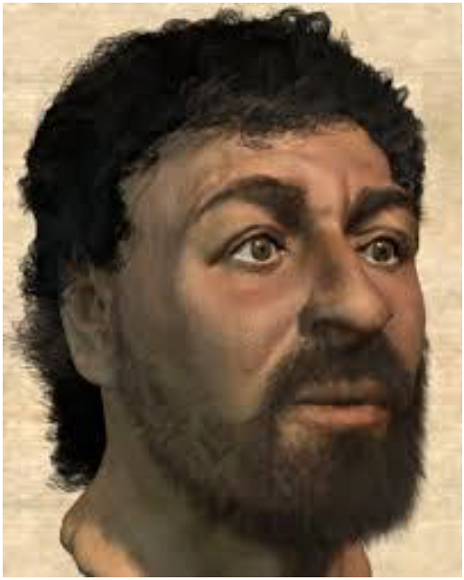
\includegraphics[scale=0.5]{graphics/jesus.PNG}
\captionof{figure}{Wie er vermutlich Aussah}
\end{minipage}
\begin{minipage}[t]{0.49\textwidth}
\centering

\includegraphics[scale=0.5]{graphics/jesus_c.PNG}
\captionof{figure}{Wie er in Büchern und Bildern aussieht}
\end{minipage}
\section{Vorlesung vom 12.03.2019}
Diese Vorlesung wurde mit einer einfachen, aber doch recht komplexen Frage eingeläutet:\\

\begin{center}
	\textbf{\large{\glqq Was ist Religion?\grqq}}
\end{center}

In der heutigen Zeit ist Religion ein recht kontroverses Thema. Wie offen darf man seine Religion in der Öffentlichkeit zeigen und was ist mit dem Begriff \textit{Religion} eigentlich gemeint? Mit der Definition der Religion gibt es da Probleme einen einheitlichen Begriff zu definieren. Der Ursprung des Begriffs könnte bei \textit{relegere} liegen, was sich etwas immer wieder zuwenden bedeutet. Übertragen auf die Religion ist damit ein genaues Einhalten von religiösen Handlungen wie Gebete oder Rituale gemeint. Andernfalls könnte der Begriff auch von \textit{religare} abstammen, was soviel wie verbinden oder anbinden umschreibt. Hier wird das Verbunden-Sein des Menschen mit einer transzendenten Wirklichkeit assoziiert. \\

In einer Gruppenarbeit mussten wir uns einer Definition von verschiedenen bekannten Persönlichkeiten zuordnen\footnote{es waren sechs verschiedene Definitionen}. Ich entschied mich dabei für die folgende Definition:\\

\begin{center}
	\textit{\glqq Religion ist der Versuch, nichts in der Welt als fremd, 						menschenfeindlich, schicksalhaft, sinnlos anzunehmen, sondern alles, was 					begegnet, zu verwandeln, einzubeziehen in die eigene menschliche Welt.\grqq}
\end{center}
\begin{flushright}
	DOROTHEE SÖLLE\\
\end{flushright}

Dies ist eine recht weltoffene Definition, welche die Religion selbst nur als Versuch für die Einbindung des Umfelds in die eigene Welt des Individuums beschreibt. Die Religion soll dem Leben und dem was darin passiert eine tiefere Bedeutung, einen Sinn zuteilen. Es ist aber auch zu erkennen, dass die Verfasserin des Zitats auch etwas auf die Nächstenliebe baute. Dies zeigt sich in der Aussage \textit{\glqq [...] nichts in der Welt als fremd, menschenfeindlich, [...] anzunehmen, [...]\grqq}. Daraus lässt sich schließen, dass Dorothee Sölle vermutlich eine Christin war. Nach kurzer Recherche ergab sich auch, dass sie evangelische Theologin war. Daraus bestätigt sich ihre christliche Weltansicht.\\

Als kleines Fazit lässt sich somit sagen, dass es keine einheitliche, allumfassende Definition von Religion gibt. Sie befasst sich mit mehr als nur einer gläubigen Verehrung eines Gottes, sondern ist ein hochkomplexes, vielschichtiges Phänomen. Diesem in der Vorlesung erwähnten Fazit stimme ich vollends zu, da es schier unmöglich scheint alle verschiedenen Interpretationen in einer einzigen Definition zu vereinen.\\
\section{Vorlesung vom 19.03.2019}
Zu dieser Vorlesung habe ich keine Notizen, da ich leider nicht anwesend war. Deshalb werden nur die Inhalte der Folien reflektiert. Behandelt wurde das Thema \textit{\glqq Einführung in den Islam\grqq}. \\

Was für mich interessant scheint, ist der Ruf \textit{\glqq All\={a}hu akbar\grqq}, welcher Übersetzt \textit{Gott ist gross (grösser)} bedeutet. In der heutigen Welt wird dieser Ruf von der Allgemeinheit aber meist einem Terrorakt zugeordnet. Grund dafür ist die Verwendung des Rufes von islamistischen\footnote{zumindest was von den Medien behauptet wird} Terrorgesellschaften vor einem Anschlag. \\

Der Islam wird in drei Grade unterteilt:
\begin{enumerate}
	\item 	Die ganze Schöpfung ist Gott
			hingegeben, insofern Gott alles
			kontrolliert\\
	\item 	Jeder, der sich Gott hingibt,
			praktiziert Islam. Deshalb war 					u.a. schon Abraham Muslim\\
	\item 	Erst im engsten Sinne bezeichnet
			Islam die Religion, wie sie durch
			Muhammad im Koran offenbart worden 			ist.\\
\end{enumerate}

Dabei werden auch die Begriffe \textit{Islam}, \textit{Muslim} und \textit{Salam} unterschieden. \textit{Islam} ist abstammend vom Verb \textit{aslama}, was soviel wie \textit{sich hingeben/unterwerfen} bedeutet. Eine Partizipialform davon ist der Begriff \textit{Muslim} und bedeutet, \textit{der, der sich Gott hingibt}. Er bezieht sich also eher auf ein Individuum, welches den Islam auslebt. \textit{Salam} beschreibt den Frieden, welcher durch die Hingabe erlangt wird.\\

Der Koran steht im Mittelpunkt des islamischen Glaubens und hat \textit{Gott} darin manifestiert. Er ist die Grundlage aller traditionellen islamistischen Kulturen, den seine Worte prägen die Gebete, sowie er auch essentiell für das Identitätskonstrukt der Muslimen ist. Ein muslimisches Sprichwort besagt:\\

\begin{center}
	\textit{\glqq Der Koran ist ein 				sprechendes Universum und das Universum 		ein schweigender Koran.\grqq}\\
\end{center}

Der Begriff \textit{Koran} stammt von \textit{qara's} ab, was soviel wie \textit{vortragen} bedeutet. Nach muslimischen Glauben ist der Koran eine Rezitation der vom Erzengel Gabriel an Muhammad eingegebenen Worten. Er besteht aus 114 Suren und ist mit Ausnahme der ersten Sure (die Fatiha) der Länge nach geordnet. Zudem sind inhaltlich viele biblische Geschichten verarbeitet. \\
\section{Vorlesung vom 26.03.2019}
Bei der heutigen Vorlesung hatten Christoph Urich, Marius Hasler und ich unsere Präsentation. Mein Teil bezog sich hauptsächlich auf ein Textstück von dem berühmten Philosophen Immanuel Kant, welcher sich mit der \textit{aufgeklärten Welt} auseinandersetzte. Allerdings möchte ich mehr auf den im Unterricht behandelten Stoff und nicht auf die Präsentation eingehen.\\

Das behandelte Thema passte zu unserer Präsentation und befasste sich mit:\\
\begin{itemize}
	\centering
	\item[ ] \glqq \textit{Was ist Aufklärung?}\textit{ Was ist Vernunft?}\grqq\\
\end{itemize}

Für die \textit{Vernunft} existiert das klassische Model. \glqq Der Mensch besitzt Vernunft\grqq. Hier wird die Vernunft als wesentlicher Bestandteil der menschlichen Seele gesehen. Aus \textit{vernünftig sein} wird geschlossen, dass die Dinge beweisbar wahr sein müssen. Es wird ein wissenschaftlich geführter Beweis benötigt, um etwas als Wahr zu bekennen. Hier ist noch wichtig zu erwähnen, dass bei der wissenschaftlicher Beweisführung die Reproduzierbarkeit eine zentrale Rolle spielt. Wo für mich auch ein kleines Problem/Widerspruch entsteht, denn einige Dinge sind nicht immer reproduzierbar. \\

Das zeitgenössische Model widerspiegelt die Vernunft so, dass im Menschen selbst die Vernunft angelegt ist. Damit ist gemeint, dass der Mensch lediglich die Möglichkeit zu vernünftigen Denken und Handeln hat. Was bedeutet, dass der Mensch zwangsläufig nicht immer vernünftig handelt. Allerdings gibt es auch hier einige Widersprüche. Nämlich teilen nicht alle Völker, Länder und sonstige Gruppierungen dieselbe Ethik/Moral. Was uns dann zum Problem führt, das \textit{vernünftige Handeln} für alle gleich zu definieren. Offensichtlich ist dies nicht möglich, denn nicht einmal in der Nahrungsaufnahme kann dies einheitlich betrachtet werden. Zum Beispiel sind für Hindus die Kühe heilig und es wäre äusserst unvernünftig für sie, eine Kuh zu verletzen, geschweige denn, sie zu essen. In den westlichen Ländern wie hier in der Schweiz ist dies allerdings kein Problem. Dies führt mich selbst zum Schluss, dass nur der Begriff \textit{Vernunft} definiert werden kann, nicht aber ob ein Mensch vernünftig handelt oder nicht. Dazu müsste die Moral mit der dieser Mensch aufwuchs und auch die Erfahrungswerte desjenigen berücksichtigt werden, um zu urteilen.\\

Im weiterführenden Unterricht wurde eine \textit{Revision} des klassischen Vernunftverständnisses erläutert. Dafür möchte ich gerne die Aussage \glqq \textit{Es ist unmöglich, durch Beweise zu absolut sicherem Wissen zu gelangen}\grqq\;aufgreifen. In der wissenschaftlichen Beweisführung wird immer mit Modellen gearbeitet. In diesen Modellen werden nur die wichtigsten Grössen berücksichtigt, wie auch deren Bedingungen. Es kann also nicht möglich sein zu absolut sicherem Wissen zu gelangen, wenn Modelle zum vereinfachten Verständnis der Dinge mit bestimmten Bedingungen benutzt werden\footnote{zu erwähnen ist, dass hier das Schlüsselwort \textbf{absolut} ist}. Dazu müsste alles zu allen Bedingungen berücksichtigt werden.\\

Für die Vernunft wurde ein Fazit festgehalten. \\
\begin{itemize}
	\item Es gibt keine zweifelsfreie absolute Wahrheit\\
	\item Vernünftiges Denken $\rightarrow$ Annäherung an die Wirklichkeit\\
	\item Überzeugungen können wahr sein, aber es ist genauso gut möglich, dass wir uns irren\\	
\end{itemize}
Mit diesem Fazit stimme ich überein. Die Gründe, weshalb ich dies auch so sehe, habe ich oben in den Absätzen bereits vermerkt.\\
\section{Vorlesung vom 02.04.2019}
Das behandelte Hauptthema heute war \textbf{Naturwissenschaft und Religion}. Als erstes ist es sinnvoll, das Verhältnis dieser beiden zu definieren, rsp. welche Fragen die beiden versuchen zu erklären.\\

\paragraph{Naturwissenschaften}
Der Mensch versucht, die Welt zu verstehen. \textbf{Wie} funktionieren die Dinge und was sind die Gesetzmäßigkeiten der Natur?\\

\paragraph{Religion}
Der Mensch versucht seinen Platz in der Welt zu finden. Was ist der Sinn des Lebens? \textbf{Warum} geschehen Dinge?\\

Die für mich interessanten Aspekte in dieser Vorlesung waren die Konflikte, welche zwischen den Naturwissenschaften und der Religion entstanden. Früher waren diese beiden stark miteinander verwoben. Wurden allerdings Forschungen ohne Einwilligung der Kirche gemacht, ging die Kirche sehr makaber damit um\footnote{z.B. mit Verbrennung}. Es wurden einige renommierte Wissenschaftler mit ihren Bewusstseins veränderlichen Hypothesen kurz angeschnitten.\\


\begin{tabular}{llll}
	Nikolaus Kopernikus & (1473-1543) & $\rightarrow$ & offenes
	heliozentrisches Weltbild \\ 
	Galileo Galilei  & (1564-1642) & $\rightarrow$ & erste überzeugende Argumente für 			physikalische\\
 	 & & &  Realität des heliozentrischen Weltbildes \\
	Isaac Newton & (1643-1727) & $\rightarrow$ & 3 Axiome der Mechanik und
	Gravitationsgesetz \\ 
	Charles Darwin & (1809-1882) & $\rightarrow$ & Evolutionstheorie \\ 
\end{tabular} 

Es wurde explizit der Fall von Galileo Galilei betrachtet. Mit seinen Argumenten für das heliozentrische Weltbild wurde das Verhältnis zwischen der Kirche und der Naturwissenschaften in den Wurzeln vergiftet. Er wurde daraufhin von der Kirche verurteilt, was aber heute von der kath. Kirche als Fehler und Irrtum gesehen wird. Auch Darwins Evolutionstheorie ist voll umfänglich von der kath. Kirche anerkannt. \\

Erwähnenswert ist, dass die Naturwissenschaften und die Religionen zwei unterschiedliche Sichtweisen auf die Welt haben und somit auch verschiedene Fragen versuchen zu beantworten. Naturwissenschaften fragen nach dem \textbf{Wie} und Religionen nach dem \textbf{Warum}. Schon in früheren Einträgen in diesem Lerntagebuch wurden ähnliche Aspekte aufgegriffen. Die Beantwortung der unterschiedlichen Fragestellungen der beiden haben eine gewisse Komplexität. Während es bei den Religionen einen relativ grossen Interpretationspielraum der Antworten gibt und es keine eindeutige universelle Antwort auf die Fragen hat, sind die Antworten bei den Naturwissenschaften evidenzbasierend und müssen empirisch beweisbar sein. Dadurch ist es schwierig, beide miteinander zu vergleichen, da sie sich meiner Meinung nach nicht mit demselben befassen und eine andere Orientierung haben. Die Religion verfolgt keine quantifizierbare, logisch nachvollziehbare Antworten. Es sind komplementäre Sichtweisen der Wirklichkeit.
\section{Vorlesung vom 09.04.2019}
Als heutiges Thema befassten wir uns mit dem \textit{Atheismus}. Dabei kam zuerst die Religionskritik und deren Formen zur Sprache. Es gibt die interne, interreligiöse und die externe Religionskritik. Die Interne gab es schon immer. Zum Beispiel kritisierte Jesus die buchstabenhörige und ausgrenzende Auslegung der Tora und betonte den in ihr enthaltenen Geist der Menschenfreundlichkeit oder Buddha kritisierte das Kastenwesen und die Göttervorstellungen zugunsten einer egalitären Gesellschaft und einer experimentellen Wirklichkeitserfahrung. Allerdings wurde nur sehr selten der Gottesglaube an sich in Frage gestellt.\\

Die interreligiöse Religionskritik ergibt sich aus der wechselseitigen Konkurrenz der Religionen in der theologischen Kontroverse. Religionsgeschichtlich finden wir diese in spezifischer Weise bei den Religionen \textit{Christentum} und \textit{Islam}. \\

Die populäre Religionskritik im 21. Jahrhundert ist der \textit{neue Atheismus}\footnote{ich interpretiere diesen als externe Religionskritik}. Dieser stammt vor allem aus den USA durch die Besiedlung der USA durch Glaubensflüchtlinge, oder auch Pilgerväter, aus Europa. \\

Neu an dieser Art von Atheismus ist z. B. das Outing nach dem Vorbild der Homosexuellen, sowie die naturwissenschaftliche Argumentation mit einer naturwissenschaftlichen Religionstheorie, der Ethik, welche explizit wissenschaftlich begründet wird usw.\\

Noch erwähnen möchte ich \glqq \textit{The four horsemen}\grqq. Es geht um vier Vertreter des \textit{neuen Atheismus} und bezeichnen sich selbst als die vier Reiter. Damit referieren sie auf die vier apokalyptischen Reiter aus der Johannesoffenbarung Kap. 6.\\

\begin{itemize}
	\item Daniel Dennett\\
	\item Sam Harris\\
	\item Christopher Hitchens\\
	\item Richard Dawkins\\
\end{itemize}

Ich selbst kann mich mit diesem \textit{neuen Atheismus} nicht identifizieren. Es macht den Eindruck, dass diese Bewegung ein ähnliches Ziel verfolgt wie die Religionen. Einfach ohne Götter und transzendente Wirklichkeiten, sondern mittels Empirismus und Rationalismus. Es wird behauptet, dass alles existierende logisch erklärbar ist. Wie es auch John Lennox im Video sagte, beinhaltet dies auch einen Glauben. Nur bin ich auch der Meinung, dass der menschliche Verstand schlicht zu klein ist um alles logisch zu erfassen. Viele Dinge sind in unserer begrenzten Vorstellung unmöglich und somit unbeweisbar. Den schliesslich denken wir in Modellen, welche nur das erfassen, was wir kennen.\\
\section{Vorlesung vom 16.04.2019}
In der heutigen Vorlesung war ich nicht anwesend. Trotzdem werde ich kurz ein paar, für mich relevanten, Themen im Lerntagebuch reflektieren.\\

Das Hauptthema war \textit{Der verantwortungsvolle Umgang mit technologischen Innovationen und Entwicklungen}. Dabei stellen sich schnell einige ethische Fragen bezüglich des enormen technologischen Fortschritts.\\

\begin{itemize}
	\item [ ] Wie sollen wir mit neuen technologischen Entwicklungen
umgehen?\\
	\item [ ] Welche Folgen haben sie – für uns als Einzelne und als
Gesellschaft?\\
	\item [ ] Wie können wir z.B. die Digitalisierung der Arbeitswelt
verantwortungsvoll gestalten?\\
\end{itemize}

Diese Fragen können nicht einfach so beantwortet werden, weil sie abhängig sind von der Ethik und Moral der Individuen. Zudem stellt sich auch das Problem, dass wenn die Digitalisierung in allen Berufsdomänen der Arbeitswelt weiter voranschreitet, steigt die Arbeitslosenzahl ins unermessliche. Dies würde bedeuten, dass das Volk auch kein Geld mehr verdient. Was würde dann geschehen?\\

Die Ethik\footnote{Orientierungswissenschaft} beschäftigt sich grundsätzlich mit der Fragen nach dem guten und gerechten Leben. Die Moral mit der Summe der Traditionen und Werten die in einer Gesellschaft gelebt und hochgehalten werden. Diese Grundsätze können religiös fundiert sein, müssen es aber nicht.\\

Leider muss ich bei gewissen Aussagen auf den Folien intervenieren. Dass...
\begin{itemize}
	\item[ ] Maschinen die Frage über Leben und Tod \textbf{nur} so behandeln können, wie die Frage ob es warm oder kalt im Raum ist,\\
	\item[ ] künstliche Intelligenz sich \textbf{nicht} fragt, ob ein Krieg gerechtfertigt ist oder ob es in einer konkreten Situation Alternativen zu einer tödlichen Aktion gibt,\\
	\item[ ] Maschinen \textbf{kein} Gewissen haben, \textbf{kein} Mitleid empfinden, töten, \textbf{ohne} den
Wert des Lebens zu anerkennen und für ihre Handlungen keine Verantwortung übernehmen,\\
\end{itemize}
sind gänzlich kontroverse Meinungen zum technologische Fortschritt und bilden eine Analogie zu der Filmreihe \textit{Terminator}\footnote{ich möchte hier lediglich eine neutrale Meinung dazu äussern}. Maschinen sind rein deterministisch funktionierende Systeme. Somit kann in der Entwicklung dieser auf genau jene Dinge reagiert werden, damit auch sie allenfalls nach einer bestimmten Moral funktionieren. Zudem stelle ich mir die Frage, wenn wir Menschen tatsächlich eine echte, \textbf{selbst denkende} und lernfähige \textit{Intelligenz} \glqq erschaffen\grqq\;(nicht eine dieser heutigen pseudo KI's in Handys und anderen Geräten), würde diese dann nicht auch beginnen, sich dieselben essenziellen Fragen über deren Existenz und Sinn des Daseins stellen? Denn wäre dies der Fall, was meiner Meinung nach möglich sein könnte, dann wären diese Maschinen sehr wohl in der Lage, anders auf die oben zitierten Aussagen zu reagieren. Wenn nicht sogar in menschlicher Art und Weise.\\
%%---BIBLIOGRAPHY------------------------------------------------------------------------
{\sloppypar
\printbibliography[heading=bibintoc]
\label{sec:lit}
%\selectlanguage{english}				%ngerman or english
%\printbibliography[heading=bibintoc]
}

%%---APPENDIX----------------------------------------------------------------------------
%\include{sections/appendix}

%%---NOTES for DEBUG---------------------------------------------------------------------
\ifdraft{%Do this only if mode=draft
%%requires \usepackage{todonotes})
\newpage
%\listoftodos[\section{Todo-Notes}]
\clearpage
}
{%Do this only if mode=final
}
\end{document}
